\section{Citing uPrime}

If \href{https://cmdrryder.github.io/uPrime/}{uPrime} contributes to your research, please cite:

\begin{quote}
\textbf{Note:}
Jibu Tom Jose, \& Ram, O. (2026). \textit{uPrime: Open-source software for velocity field and turbulence analysis from PIV and CFD data}. Transient Fluid Mechanics Laboratory (TFML), Technion (v0.8.0-alpha). Zenodo.\\
\url{https://doi.org/10.5281/zenodo.19376184}
\end{quote}

The citation text and DOI are also accessible directly from within the application via `About uPrime` at the bottom of the sidebar. The DOI can be copied to the clipboard using the copy button next to it.

\begin{figure}[htbp]
  \centering
  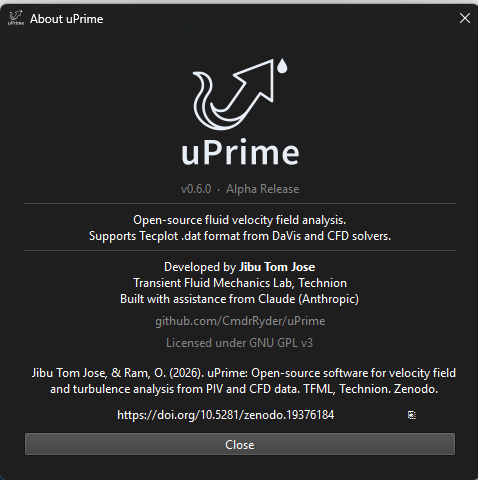
\includegraphics[width=0.5\linewidth]{fig_about}
  \caption{About \href{https://cmdrryder.github.io/uPrime/}{uPrime} dialog (v0.8.0). The citation text and DOI are displayed with a one-click copy button. The GitHub link opens the repository in the default browser.}
  \label{fig:about}
\end{figure}

